\begin{columns}[T]
  \begin{column}[T]{.25\textwidth}
We show processing of a modulo 4 computation:
  \begin{itemize}
    \item The left figure shows the input flow graph.
    \item The table visualises how instructions (cells) are fused together across different data sets (represented by indices).
    \item The next block shows results produced for the example table. We can see a vectorised and a nonvectorised output fragment. Lines 3,5 and 6 of the vectorised fragment show needed width conversions, e.g., joining outputs of two LD instructions into a single vector.
    \item The last block shows an example output file.
  \end{itemize}
\ 
\end{column}
  \begin{column}[T]{.70\textwidth}


  \begin{longtable}{ m{4cm} m{2cm} m{9cm} m{2cm} m{18cm} m{2cm} m{15cm} }

%\begin{minipage}{8cm}
%\begin{verbatim}
%int mod(int a)
%{
%  return a % 4;
%}
%\end{verbatim}
%\end{minipage}
%&

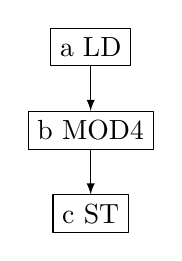
\begin{tikzpicture}[>=latex,line join=bevel,]
%%
\node (a) at (0bp,70bp) [draw,rectangle] {a LD};
  \node (c) at (0bp,10bp) [draw,rectangle] {c ST};
  \node (b) at (0bp,40bp) [draw,rectangle] {b MOD4};
  \draw [->] (a) -- (b);
  \draw [->] (b) -- (c);
%
\end{tikzpicture}


&
$\rightarrow$
&
\begin{minipage}{11.5cm}
\begin{tabular}{c|c|c|c|c|c|}
\cline{2-6}
a (LD) & 1 & 2 & 3 & 4 & ...\\
    \cline{2-6}
    b (MOD4) & \multicolumn{2}{c|}{1-2} & \multicolumn{2}{c|}{3-4} & ... \\
      \cline{2-6}
      c (ST) & 1 & 2 & 3 & 4 & ...\\
        \cline{2-6}
        \end{tabular}

        \end{minipage}
&
$\rightarrow$
        &
        \begin{minipage}{23cm}
\begin{verbatim}
uint16_t a = input_a[i++];
uint16_t b = a % 4;
output_c[j++] = b;

uint16_t a_0 = input_a[i++];
uint16_t a_1 = input_a[i++];
uint32_t a_conv0 = a_0 | (a_1 << 16);
uint32_t b = a_conv0 & 0x00030003;
uint16_t b_conv0 = b & 0xFFFF;
uint16_t b_conv1 = (b & 0xFFFF0000) >> 16;
output_c[j++] = b_conv0;
output_c[j++] = b_conv1;
\end{verbatim}
\end{minipage}
        &
        $\rightarrow$
        &
        \begin{minipage}{23cm}
\begin{verbatim}
void f(uint16_t** input_a,
       uint16_t** output_c,
       int count)
{
  int i = 0;
  int j = 0;
  for(; count >= 2; count -= 2)
  { <vectorised fragment> }
  for(; count >  0; count--)
  { <nonvectorised fragment> }
}

\end{verbatim}
        \end{minipage}

        \end{longtable}
        \end{column}
        \end{columns}
